Como muestra la figura \ref{fig:pc_uc_motors}, solo se controlan dos motores, y
para mejor precisi\'on y mantener el dise\~no compatible con impresoras viejas
matriz de punto, los motores \emph{paso a paso} son la mejor elecci\'on.\\

Existen dos grandes tipos de motores paso a paso; \emph{bipolares} y
\emph{unipolares}. La figura \ref{fig:stepper_motors} muestra la disposici\'on
y conexi\'on de los devanados de ambos tipos de motores. 


%http://www.electojects.com/motors/02440.gif
\begin{figure}[htp]
\centering
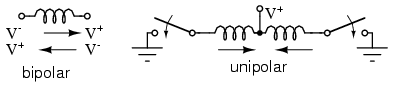
\includegraphics[scale=0.7]{./img/02440.png}
\caption{Motores paso a paso.}
\label{fig:stepper_motors}
\end{figure}

Claramente la desventaja que presentan los motores \emph{bipolares} frente a
los \emph{unipolares} es que necesitan invertir el sentido de la corriente en
sus bobinados, esto implica mayor complejidad en el circuito controlador.\
Y en contra partida la mayor ventaja de los motores \emph{unipolares} radica
(m\'as all\'a de la simpleza del circuito controlador) en que eran los m\'as
usados\footnote{Y son m\'as f\'aciles de encontrar en el mercado local} en la
antiguas impresoras matriz de punto, lo cual es un beneficio m\'as que
importante
para este trabajo.\\

Para satisfacer los dos movimientos mec\'anicos necesarios (rotaci\'on del
rodillo de papel y desplazamiento horizontal del cabezal) el dise\~no requiere
controlar dos motores paso a paso unipolares individuales.\
Entre los motores paso a paso \emph{unipolares}, los m\'as usados son los de
cuatro fases, m\'as com\'unmente denominados \emph{motor de cinco cables}. La
figura \ref{fig:stepper_motor_5_wire} muestra simb\'olicamente la
distribuci\'on interna de los devanados de este tipo de motores.

% http://www.piclist.com/images/member/RB-ezy-Q33/5wire.GIF
\begin{figure}[htp]
\centering
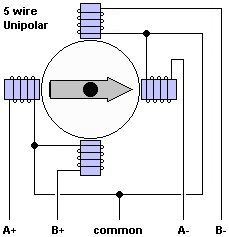
\includegraphics[scale=0.5]{./img/5wire.png}
\caption{Motor unipolar paso a paso de 4 fases.}
\label{fig:stepper_motor_5_wire}
\end{figure}

Para lograr la rotaci\'on, cada bobina debe ser energizada de forma
independiente y siguiendo una secuencia particular. El circuito de la figura
\ref{fig:cir_single_coil} satisface los requisitos m\'inimos para energizar una
\'unica bobina.

\begin{figure}[htp]
\centering
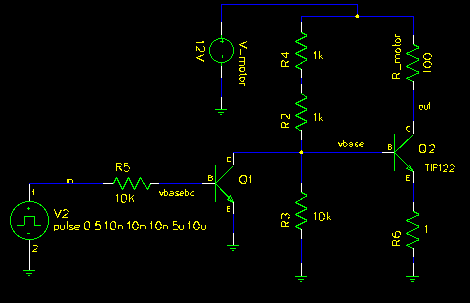
\includegraphics[width=11cm]{./img/cir_single_coil.png}
\caption{Circuito de potencia para una bobina de motor paso a paso unipolar.}
\label{fig:cir_single_coil}
\end{figure}

El divisor resistivo \emph{R2 R3} es una resistencia variable, que junto con
la resistencia de emisor de 1 \ohm  permiten controlar la corriente que circula
por la bobina, de esta manera este circuito puede ser ser usado por diversos
motores de diversas impedancias. Debido a que el el circuito de salida se
conecta directamente a la bobina del motor, y esta puede ser de muy baja
impedancia, el transistor de salida debe ser capaz de manejar corrientes altas,
en este caso se hace uso de un \emph{TIP122}.\
La figura \ref{fig:cir_single_coil_plot} muestra las diferentes tensiones que
act\'uan en el circuito. 

\begin{figure}[htp]
\centering
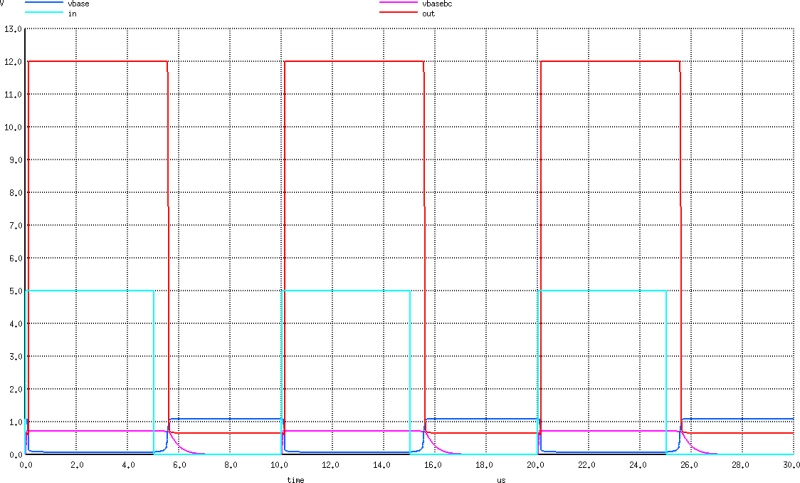
\includegraphics[width=15cm]{./img/cir_single_coil_plot.png}
\caption{Simulaci\'on del circuito de potencia para una bobina de motor paso a
paso unipolar.}
\label{fig:cir_single_coil_plot}
\end{figure}

Un motor paso a paso unipolar de cuatro fases tiene cuatro bobinas, para
manejar los dos motores es necesario luego replicar ocho veces este circuito.
El esquem\'atico final se encuentra en el anexo en
\fullref{cap:driver_schema}.\\

